%!TeX root=./ordenacao.tex

%% ------------------------------------------------------------------------- %%


\section{Lista ordenada cinética}
\label{sec:lista}
Um jeito natural de resolver o problema da ordenação cinética é por
meio de uma lista ordenada cinética, que é manter um vetor com os
elementos dados em ordem decrescente do valor no instante atual.

Inicialmente o vetor começa com os valores dos elementos no instante
$t = 0$, ou seja, com o valor $x_0$ de cada elemento, e este vetor é
ordenado em ordem decrescente.
Na verdade, o vetor pode armazenar não os valores, mas os índices dos elementos, e fazemos
ordenação indireta.
No caso de empates nos valores dos elementos, o desempate
será feito pela velocidade, ou seja, se dois elementos, digamos $i$
e $j$, possuem o mesmo valor $x_0$, mas a velocidade de $i$ é maior
que a de $j$, então $i$ será tratado como se possuísse maior valor
que $j$ no instante inicial.
Esse mesmo critério de desempate será aplicado em todos os instantes e também em todos os problemas daqui
em diante.

Uma vez de posse do vetor ordenado com os valores iniciais
decrescentemente, construímos um certificado para cada par de
elementos consecutivos no vetor.
O $i$-ésimo certificado, denotado pelo par $(i, t)$, se refere ao par das posições $i$ e $i + 1$.
O valor $t$ consiste no instante de tempo em que o $i$-ésimo elemento
deixará de ter um valor maior que o valor do $(i + 1)$-ésimo
elemento do vetor, se esse instante for maior ou igual a 0, ou em
geral ao instante atual.
Do contrário, o valor $t$ consiste em$+\infty$.
O valor $t$ do certificado é o seu \textit{prazo de
validade}.

Esses prazos de validade determinam os \textit{eventos} que
potencialmente causarão modificações no vetor que mantém os
elementos ordenados pelo seu valor e consequentemente em alguns
certificados.

Esses $n - 1$ certificados são colocados em uma fila com
prioridades, com seu prazo de validade determinando a prioridade.
Estamos interessados nos certificados com menor prazo de validade.
Ou seja, a fila com prioridades pode ser implementada com um heap de
mínimo que usa os prazos de validade como chave.

Para descrever a implementação das três operações, precisamos
estabelecer o nome das variáveis usadas.
São elas:
\begin{enumerate}
    \item $n$: o número de elementos dados;
    \item $x_0$ e \textit{speed}: vetores com o valor e a velocidade
    inicial de cada um dos $n$ elementos;
    \item \now: instante atual.
    A variável \now\ será tratada como
    global, ou seja, será utilizada nas rotinas sem ser passada como
    argumento;
    \item \textit{sorted}: vetor com os índices dos $n$ elementos em
    ordem decrescente do seu valor no instante \textit{now};
    \item \textit{indS}: vetor de $n$ posições; \textit{indS}[$j$]
    guarda a posição em \textit{sorted} do elemento $j$;
    \item \textit{cert}: vetor com os $n-1$ certificados;
    \textit{cert}$[i]$ guarda o $i$-ésimo, ou seja, o certificado
    entre $\sorted[i]$ e ${\sorted[i+1]}$, para~$1\leq i < n$;
    \item \textit{Q}: fila que guarda os inteiros $1, \ldots, n-1$,
    sendo \textit{cert}[$i$] a prioridade de cada elemento da fila.
\end{enumerate}

A interface da fila com prioridades que utilizaremos inclui as duas
seguintes operações:
\begin{enumerate}
    \item \textsc{minPQ}$(Q)$: devolve $i$ tal que
    \textit{cert}[$i$] é mínimo;
    \item \textsc{updatePQ}$(Q, i, t)$: altera a chave do
    $i$-ésimo certificado para $t$ e ajusta $Q$ de acordo.
\end{enumerate}

O vetor $\textit{indS}$ nos permite implementar a operação
\textsc{change} de maneira eficiente, pois, dado um elemento $j$,
precisamos saber a posição $i$ do elemento $j$ em $\sorted$ para
recalcular os certificados relacionados com a posição $i$.

Para implementar a operação \textsc{updatePQ}$(Q, i, t)$ em tempo
logarítmico no número de elementos na fila $Q$, é necessário
utilizar um vetor adicional \textit{indQ} que guarda em
\textit{indQ}$[i]$ a posição em $Q$ do $i$-ésimo certificado.

Com isso, a operação \textsc{advance}$(t)$, implementada no
Algoritmo~\ref{alg:lista-ordenada:advance}, segue uma ideia bem simples: enquanto
$t$ for maior que o prazo de validade do próximo evento, avançamos
\textit{now} para esse prazo de validade e tratamos esse evento.
Nos problemas seguintes, a operação \textsc{advance}$(t)$ será sempre a
mesma;
as únicas mudanças ocorrerão no tratamento de um evento.
Um evento está associado a um certificado $(i, t)$ que expira quando
$\now = t$.
O tratamento do evento correspondente ao certificado $(i, t)$ consiste em trocar de lugar os
índices das posições $i$ e $i + 1$ do vetor \textit{sorted}, recalcular o prazo de validade do
$(i-1)$-ésimo certificado se $i > 1$, e do $(i + 1)$-ésimo
certificado se $i < n - 1$.
O $i$-ésimo certificado também deve ser ajustado para $+\infty$.
Finalmente, é necessário fazer ajustes em $Q$, nas chaves dos certificados que sofreram
alteração.

\begin{algorithm}[H]
    \caption{Função \textsc{advance}.} \label{alg:lista-ordenada:advance}
\begin{algorithmic}[1]
    \Function{advance}{$t$}
        \If{$t < $ \now}
            \State \Return
        \EndIf
        \State $i \leftarrow \Call{minPQ}{$Q$}$
        \While{$t \geq$ \cert[$i$]}
            \State \now $~\leftarrow$ \cert[i]
            \State $\Call{event}$
            \State $i \leftarrow \Call{minPQ}{$Q$}$
        \EndWhile
        \State \now $~\leftarrow$ $t$
    \EndFunction
\end{algorithmic}
\end{algorithm}

Na implementação da operação \textsc{event}, utilizaremos a rotina
\textsc{update}$(i)$ para calcular o novo prazo de validade $t$ do
$i$-ésimo certificado, se $1 \leq i < n$, e fazer os devidos ajustes
em~$Q$.
Ambas as implementações podem ser encontradas nos Algoritmos~\ref{alg:lista-ordenada:evento}
e~\ref{alg:lista-ordenada:update}, respectivamente.
Para calcular $t$, utilizaremos uma rotina chamada \textsc{expire}$(i,
j)$, que calcula o prazo de validade dos certificados entre os
elementos $i$ e $j$ no instante \now.
A rotina auxiliar \textsc{expire}$(i, j)$ não mudará para outros problemas, mantendo a
mesma definição.
As Figuras~\ref{fig:lista:expire} e~\ref{fig:lista:update} ilustram as atualizações feitas por
essas rotinas.

\begin{algorithm}[H]
    \caption{Função \textsc{update}.} \label{torneioi:update}
    \begin{algorithmic}[1]
        \Function{update}{$e$}
            \If{$e \neq$ NULL}
                \State $e'\leftarrow \torneio[(e.\lastmatch)/2]$
                \State $t \leftarrow $ \Call{expire}{$e, e'$}
                \State \Call{updatePQ}{$Q,e,t$}
            \EndIf
        \EndFunction
        % \LineComment{Em expire$(e, e')$, $e'$ pode ser nulo e
        % nesse caso o retorno é $+\infty$.}
        % \LineComment{\Call{expire}{$e,e'$} calcula a validade do
        % certificado entre os elementos $e$ e $e'$, se $e'$ é NULL
        % retorna $+\infty$}
    \end{algorithmic}
\end{algorithm}

\begin{algorithm}[H]
    \caption{Função \textsc{event}.} \label{torneioi:evento}
    \begin{algorithmic}[1]
        \Function{event}{\nnull}
            \State $e \leftarrow  $ \Call{minPQ}{$Q$}
            \While{$e.\cert$ = \now}
                \State $j \leftarrow e.\lastmatch$
                \State $k \leftarrow 2\cdot \floor{\frac{j}{2}}
                + ((j + 1)\mod2)$ \Comment{adversário}
                \While{$j > 1$ \AND \Call{value}{$j$} $\geq$
                    \Call{value}{$k$}}
                    \State \torneio[$\floor{\frac{j}{2}}$]
                    $\leftarrow~$\torneio[$j$]
                    \State $\torneio[k].\lastmatch$ $\leftarrow k$
                    \State \Call{update}{$\torneio[k]$}
                    \State $j \leftarrow \floor{\frac{j}{2}}$
                    \State $k \leftarrow 2\cdot \floor{\frac{j}{2}}
                    + ((j + 1)\mod2)$ \Comment{adversário}
                \EndWhile
                \State $\torneio[j].\lastmatch \leftarrow j$
                \State \Call{update}{$\torneio[j]$}
                \State $e \leftarrow  $ \Call{minPQ}{$Q$}
            \EndWhile
        % \LineComment{swapHeap$(i, \floor{\frac{i}{2}})$ troca \heap[$i$] por \heap$\left[\floor{\frac{i}{2}}\right]$}
        \EndFunction
%        \LineComment{\Call{compare}{$i, j$} retorna se o valor
%        de $i$ é maior que o valor de $j$.}
    \end{algorithmic}
\end{algorithm}

\begin{figure}[H]
    \centering
    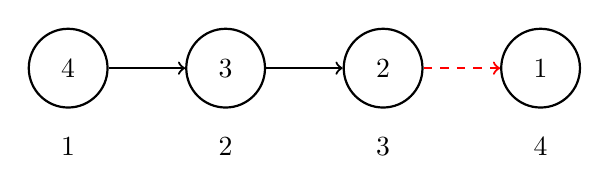
\begin{tikzpicture}[thick]
        \edef\pos{0}
        \foreach \x in {1, 2,..., 4}{
            \pgfmathparse{\pos+2}
            \xdef\pos{\pgfmathresult}
            \node  at (\pos, -1) {$\x$};
        }
        \node[circle,draw, minimum size=1cm] (1) at  (2, 0) {$4$};
        \node[circle,draw, minimum size=1cm] (2) at  (4, 0) {$3$};
        \node[circle,draw, minimum size=1cm] (3) at  (6, 0) {$2$};
        \node[circle,draw, minimum size=1cm] (4) at  (8, 0) {$1$};
        \draw[->] (1) -- (2);
        \draw[->] (2) -- (3);
        \draw[->, color=red, dashed] (3) -- (4);
    \end{tikzpicture}
    \caption[Exemplo de expiração de certificado da lista ordenada]{No exemplo da
    Figura~\ref{fig:ordenacao:exemplo}, \cert[3] expirou no instante $t = 2$.}
    \label{fig:lista:expire}
\end{figure}

\begin{algorithm}[H]
    \caption{Função \textsc{update}.} \label{torneioi:update}
    \begin{algorithmic}[1]
        \Function{update}{$e$}
            \If{$e \neq$ NULL}
                \State $e'\leftarrow \torneio[(e.\lastmatch)/2]$
                \State $t \leftarrow $ \Call{expire}{$e, e'$}
                \State \Call{updatePQ}{$Q,e,t$}
            \EndIf
        \EndFunction
        % \LineComment{Em expire$(e, e')$, $e'$ pode ser nulo e
        % nesse caso o retorno é $+\infty$.}
        % \LineComment{\Call{expire}{$e,e'$} calcula a validade do
        % certificado entre os elementos $e$ e $e'$, se $e'$ é NULL
        % retorna $+\infty$}
    \end{algorithmic}
\end{algorithm}

A operação \textsc{query\_kth}$(i)$, implementada no Algoritmo~\ref{lista:query}, consiste em
devolver \textit{sorted}$[i]$, enquanto que a operação \textsc{change}$(j, v)$ consiste em alterar
a posição $x_0[j]$ para $x_0[j] + (\mathit{speed}[j] - v)\cdot now$,
a posição \textit{speed}[j] para \textit{v} e recalcular os
eventuais certificados de que $j$ participa.
O novo valor da posição $x_0[j]$ corresponde à posição inicial do elemento caso ele tivesse
começado com essa velocidade e estivesse na posição atual agora.
Para tanto, a partir da posição $i$ em que $j$ se encontra no vetor
\textit{sorted}, podemos recalcular \textit{cert}$[i - 1]$ se $i >
1$ e \textit{cert}$[i]$ se $i < n$, como ilustrado na Figura~\ref{fig:lista:after}, acionando a
rotina \textsc{update} para fazer
os devidos acertos em~$Q$ correspondentes a estas modificações.
As instruções executadas pela operação \textsc{change} estão descritas
no Algoritmo~\ref{lista:change}.

\begin{algorithm}
    \caption{Função \textsc{query\_kth}.} \label{abb:query}
\begin{algorithmic}[1]
    \Function{query\_kth}{$i$}
        \State $node \leftarrow root$
        \State $r \leftarrow \Call{rsize}{node}$
        \While{$i \neq r + 1$}
        \If{$i \leq r$}
            \State $node \leftarrow node.right$
        \Else
            \State $node \leftarrow node.left$
            \State $i \leftarrow i - (r + 1)$
        \EndIf
        \State $r \leftarrow \Call{rsize}{node}$
        \EndWhile
        \State \Return $node.key$
    \EndFunction
\end{algorithmic}
\end{algorithm}

\begin{algorithm}
    \caption{Função \textsc{change}.} \label{lista:change}
\begin{algorithmic}[1]
    \Function{change}{$j, v$}
        \State $x_0$[$j$] $\leftarrow  x_0$[$j$]
        $+~($\speed[$j$]$~-~v)~\cdot~$\now;
        \State \speed[$j$] $\leftarrow  v$
        \State $i \leftarrow$ \inds[$j$]
        \State \Call{update}{$i$}
        \State \Call{update}{$i - 1$}
    \EndFunction
\end{algorithmic}
\end{algorithm}

\begin{figure}
    \centering
    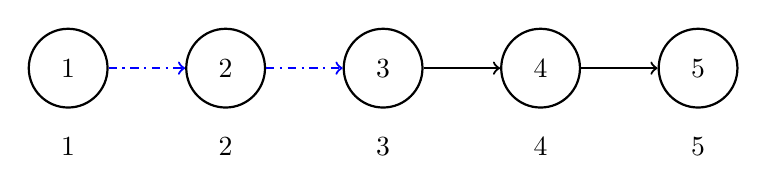
\begin{tikzpicture}[thick]
        \edef\pos{0}
        \foreach \x in {1, 2,..., 5}{
            \pgfmathparse{\pos+2}
            \xdef\pos{\pgfmathresult}
            \node[circle,draw, minimum size=1cm] (\x) at
                (\pos, 0) {$\x$};
            \node  at (\pos, -1) {$\x$};
        }
        % \foreach \x [evaluate=\x as \y using int(\x + 1)] in {1, 2,..., 4}{
        %     \ifthenelse{\x==2}{\draw[->, draw=red] (\x) -- (\y);}{\draw[->, draw=black] (\x) -- (\y);}
        % }
        \draw[->, color=blue, dashdotted] (1) -- (2);
        \draw[->, color=blue, dashdotted] (2) -- (3);
        \draw[->] (3) -- (4);
        \draw[->] (4) -- (5);
        % \draw[->] (1) edge (2) (2) edge (3) (3) edge (4) (4) edge (5)
    \end{tikzpicture}
    \caption[Certificados atualizados]{Após a mudança de velocidade
            do elemento 2, que se encontra em \sorted[2], \cert[1] e
            \cert[2] foram atualizados.}
    \label{fig:lista:after}
\end{figure}

\subsection{Análise de desempenho}\label{subsec:analise-de-desempenho}

A lista ordenada cinética é uma estrutura \textit{responsiva}, pois o custo de
processar um certificado é $O(\lg{n})$.
O custo de processar um certificado corresponde a uma iteração da linha $3$ na operação
\textsc{event}, que atualiza o vetor que guarda o índice dos elementos em $O(1)$ e realiza
alterações na fila de certificados em tempo $O(\lg{n})$, por isso o custo total $O(\lg{n})$ para
processar um certificado.

A lista ordenada cinética é uma estrutura \textit{eficiente}, pois todos os eventos
processados são eventos \textit{externos}, isto é, todo vencimento de
certificado representa a troca de ordem entre dois elementos na lista, que é uma
mudança na descrição combinatória do problema.

A lista ordenada cinética é uma estrutura \textit{compacta}, pois como cada
certificado está associado à relação de ordem entre um elemento e seu
predecessor, teremos no máximo $n$ certificados na fila de prioridades num
determinado instante.

A lista ordenada cinética é uma estrutura \textit{local}, pois cada elemento
está relacionado a no máximo dois certificados, o certificado entre ele e o
seu predecessor e o certificado entre o seu sucessor e ele.
